\documentclass[14pt, a4paper]{article}
\usepackage[russian]{babel}
\usepackage{graphicx}
% \usepackage{tabularx}
\usepackage{layout}
\usepackage[14pt]{extsizes}
\usepackage[hidelinks]{hyperref}
\usepackage{caption}

\usepackage{listings}
\usepackage{xcolor}
\usepackage{float}
\usepackage{ulem}

\setcounter{tocdepth}{4}
\setcounter{secnumdepth}{4}
\setlength{\emergencystretch}{3pt}
% \usepackage[compact]{titlesec}

\oddsidemargin = 0pt
\marginparwidth = 45pt %57
\textwidth = 467pt
\textheight = 716pt
\topmargin = 0pt %17
\footskip = 30pt %30
\headheight = 0pt %12
\headsep = 0pt %25

\title{Методичка 4}

\definecolor{codegreen}{rgb}{0,0.6,0}
\definecolor{codegray}{rgb}{0.5,0.5,0.5}
\definecolor{codepurple}{rgb}{0.58,0,0.82}
\definecolor{backcolour}{rgb}{0.97,0.97,0.97}

\lstdefinestyle{mystyle}{
    backgroundcolor=\color{backcolour},   
    commentstyle=\color{codegreen},
    keywordstyle=\color{magenta},
    numberstyle=\tiny\color{codegray},
    stringstyle=\color{codepurple},
    basicstyle=\ttfamily\footnotesize,
    breakatwhitespace=false,         
    breaklines=true,                 
    captionpos=b,                    
    keepspaces=true,
    frame=single,                 
    % numbers=left,                    
    % numbersep=5pt,                  
    showspaces=false,                
    showstringspaces=false,
    showtabs=false,                  
    tabsize=2,
    extendedchars=\true,
    inputencoding=utf8x
}

\lstset{style=mystyle, extendedchars=\true, literate=
{а}{ {\selectfont\char224} }1
{б}{ {\selectfont\char225} }1
{в}{ {\selectfont\char226} }1
{г}{ {\selectfont\char227} }1
{д}{ {\selectfont\char228} }1
{е}{ {\selectfont\char229} }1
{ё}{ {\"e} }1
{ж}{ {\selectfont\char230} }1
{з}{ {\selectfont\char231} }1
{и}{ {\selectfont\char232} }1
{й}{ {\selectfont\char233} }1
{к}{ {\selectfont\char234} }1
{л}{ {\selectfont\char235} }1
{м}{ {\selectfont\char236} }1
{н}{ {\selectfont\char237} }1
{о}{ {\selectfont\char238} }1
{п}{ {\selectfont\char239} }1
{р}{ {\selectfont\char240} }1
{с}{ {\selectfont\char241} }1
{т}{ {\selectfont\char242} }1
{у}{ {\selectfont\char243} }1
{ф}{ {\selectfont\char244} }1
{х}{ {\selectfont\char245} }1
{ц}{ {\selectfont\char246} }1
{ч}{ {\selectfont\char247} }1
{ш}{ {\selectfont\char248} }1
{щ}{ {\selectfont\char249} }1
{ъ}{ {\selectfont\char250} }1
{ы}{ {\selectfont\char251} }1
{ь}{ {\selectfont\char252} }1
{э}{ {\selectfont\char253} }1
{ю}{ {\selectfont\char254} }1
{я}{ {\selectfont\char255} }1
{А}{ {\selectfont\char192} }1
{Б}{ {\selectfont\char193} }1
{В}{ {\selectfont\char194} }1
{Г}{ {\selectfont\char195} }1
{Д}{ {\selectfont\char196} }1
{Е}{ {\selectfont\char197} }1
{Ё}{ {\"E} }1
{Ж}{ {\selectfont\char198} }1
{З}{ {\selectfont\char199} }1
{И}{ {\selectfont\char200} }1
{Й}{ {\selectfont\char201} }1
{К}{ {\selectfont\char202} }1
{Л}{ {\selectfont\char203} }1
{М}{ {\selectfont\char204} }1
{Н}{ {\selectfont\char205} }1
{О}{ {\selectfont\char206} }1
{П}{ {\selectfont\char207} }1
{Р}{ {\selectfont\char208} }1
{С}{ {\selectfont\char209} }1
{Т}{ {\selectfont\char210} }1
{У}{ {\selectfont\char211} }1
{Ф}{ {\selectfont\char212} }1
{Х}{ {\selectfont\char213} }1
{Ц}{ {\selectfont\char214} }1
{Ч}{ {\selectfont\char215} }1
{Ш}{ {\selectfont\char216} }1
{Щ}{ {\selectfont\char217} }1
{Ъ}{ {\selectfont\char218} }1
{Ы}{ {\selectfont\char219} }1
{Ь}{ {\selectfont\char220} }1
{Э}{ {\selectfont\char221} }1
{Ю}{ {\selectfont\char222} }1
{Я}{ {\selectfont\char223} }1
}


\begin{document}

\begin{titlepage}
    \topmargin=216pt
    \newpage
    \hangindent=0.7cm
    \huge ИУ-10\\
    Системное\\
    Программное\\
    Обеспечение\\
    \textbf{Модуль 2\\ 
    Веб-сервер Apache}

    \vspace{10cm}

    \begin{center}
        \small\textit{Москва, 2022}
    \end{center}
\end{titlepage}
\tableofcontents
\newpage



\section*{Apache}
\addcontentsline{toc}{section}{Apache}
Интернет невозможно представить без всевозможных сайтов. Все они работают за счёт веб-серверов 
– программ, отвечающих за передачу данных от физических хранилищ до браузеров пользователей.

Веб-сервер работает в качестве «посредника» между пользователем и физическим сервером. 
При получении запроса от посетителя он ищет необходимую страницу в каталоге с сайтом и 
отправляет её в ответ. Браузер принимает полученный файл, обрабатывает его и отображает на экране посетителя.

Передача информации веб-сервера выполняется по протоколу \textbf{HTTP} (\textbf{HyperText Transfer Protocol}), 
изначально созданного для работы с \textbf{HTML}-страницами. Уже позже стало возможным отправлять через 
\textbf{HTTP} файлы любых типов. В последнее время преобладают сайты, работающие через \textbf{HTTPS}. Это улучшенная 
версия HTTP, которая отличается от предшественника тем, что поддерживает шифрование трафика \textbf{TLS/SSL} 
между пользователем и сервером.

Звание самого популярного веб-сервера в мире уже более 25 лет удерживает за собой \textbf{Apache HTTP Server}, 
который принято называть сокращенно \textbf{Apache} или «\textbf{Апач}». Сегодня программа обслуживает более 40\% всех 
существующих серверов, включая проекты \textbf{IBM}, \textbf{eBay}, \textbf{PayPal} и \textbf{Facebook}.

Рассмотрим причины популярности \textbf{Apache} подробнее. Это не только пополнит копилку знаний об 
интернет-технологиях, но и поможет сделать правильный выбор веб-сервера для размещения сайта в будущем.



\subsection*{Что это такое}
\addcontentsline{toc}{subsection}{Что это такое}

\textbf{Apache} – это свободное программное обеспечение для размещения веб-сервера. Он хорошо показывает 
себя в работе с масштабными проектами, поэтому заслуженно считается одним из самых популярных 
веб-серверов. Кроме того, \textbf{Apache} очень гибок в плане настройки, что даёт возможность реализовать 
все особенности размещаемого веб-ресурса.

\subsubsection*{История создания}
\addcontentsline{toc}{subsubsection}{История создания}
Apache HTTP Server был выпущен в 1995 году разработчиком Робертом Маккулом из Университета штата 
Иллинойс (UIUC). Продукт возник как доработанная версия другого HTTP-клиента – NCSA HTTPd 1.3, 
созданного Робертом ранее.

Основой для модификации стали многочисленные «патчи» или программные «заплатки» для NCSA. 
Именно отсюда (а не от индейского племени апачей) изначально и происходит название Apache.
Оно расшифровывается как «a patchy server» или «сервер с патчами».

\begin{figure}[h]%current location
    \centering
    \scalebox{1}{
\includegraphics[width=0.8\textwidth]{imgs/1.0.jpg}}
    \label{1.0}
\end{figure}

Разработкой и поддержкой продукта с 1999 года занимается организация \textbf{Apache Software Foundation} 
(\textbf{\uline{ASF}}) – сообщество экспертов-энтузиастов со всего мира. Этим же некоммерческим фондом была 
создана официальная лицензия ПО – \textbf{Apache License}.

В 2000 году ASF представило новую версию Apache 2.0 с полностью переработанной архитектурой, 
свободной от кода NCSA. С этого момента веб-сервер развивается по двум основным веткам – 1.х и 2.х.

\subsection*{Как устроен Apache}
\addcontentsline{toc}{subsection}{Как устроен Apache}

\begin{figure}[h]%current location
    \centering
    \scalebox{1}{
\includegraphics[width=0.495\textwidth]{imgs/1.1.jpg}}
    \scalebox{1}{
\includegraphics[width=0.495\textwidth]{imgs/1.2.jpg}}
    \label{1.1, 1.2}
\end{figure}

\subsubsection*{Архитектура}
\addcontentsline{toc}{subsubsection}{Архитектура}
Apache состоит из ядра и динамической модульной системы. Параметры системы 
изменяются с помощью конфигурационных файлов.


\subsubsection*{Ядро}
\addcontentsline{toc}{subsubsection}{Ядро}
Ядро Apache разработано Apache Software Foundation на языке C. Основные функции — обработка 
конфигурационных файлов, протокол HTTP/HTTPS и загрузка модулей. Ядро может работать без модулей, 
но будет иметь ограниченный функционал.

\subsubsection*{Модульная система}
\addcontentsline{toc}{subsubsection}{Модульная система}
Модуль – отдельный файл, подключение которого расширяет изначальный функционал ядра. Они могут 
включаться в состав ПО при первоначальной установке или подгружаться позже через изменение конфигурационного файла.

Большинство из них отвечает за определенный аспект обработки клиентского запроса – поддержку различных 
языков программирования, безопасность, кэширование, аутентификацию и т.д. Таким образом, большая 
задача разбивается на несколько фаз, каждую из которых решает отдельный, узкоспециализированный модуль.

Для Apache существует больше 500 модулей. Многие популярные веб-приложения сразу выпускаются в виде 
модуля к Apache. Например, \linebreak ISPmanager и VDSmanager.


\subsubsection*{Конфигурация}
\addcontentsline{toc}{subsubsection}{Конфигурация}
Система конфигурации Apache работает на текстовых файлах с прописанными настройками. Она подразделяется на 
три условных уровня, для каждого из которых имеется свой конфигурационный файл:

\begin{enumerate}
    \item Уровень конфигурации сервера (файл \textbf{httpd.conf}) – основной конфигурационный файл. 
    Действпространяется на весь механизм веб-сервера.
    \item Уровень каталога (файл \textbf{.htaccess}) – дополнительный конфигурационный файл. Его 
    директватывают только каталог, где расположен файл, а также вложенные подкаталоги.
    \item Уровень виртуального хоста (файл \textbf{httpd.conf}> или \textbf{extra/httpd-vhosts.conf}).
\end{enumerate}

Обычно конфигурационные файлы Apache находятся в папке «conf», а дополнительные конфигурационные файлы 
во вложенной в нее папке «extra». Внести изменения можно как через редактирование самого файла, так и 
через командную строку.

\subsubsection*{Виртуальные хосты}
\addcontentsline{toc}{subsubsection}{Виртуальные хосты}
Веб-хост – это компонент сервера, отвечающий за обслуживание одного размещенного на нем 
объекта (сайта, виртуального сервера). Система виртуальных хостов Apache позволяет одновременно 
запускать несколько проектов с одного IP-адреса.

В Apache можно установить настройки модуля и ядра, а также вводить лимиты на потребление серверных 
ресурсов (трафик, RAM, CPU) для каждого виртуального хоста в отдельности. Это технологическая основа 
всего механизма веб-хостинга.


\subsection*{Достоинства и недостатки Apache}
\addcontentsline{toc}{subsection}{Достоинства и недостатки Apache}
\textbf{Плюсы}
\begin{itemize}
    \item \textbf{Доступность}. Это программное обеспечение с открытым исходным кодом. Значит, его 
    может бесплатно использовать или модифицировать любой желающий. Разработчики по всему миру 
    создают конфигурации и модули веб-сервера для своих специфических нужд. По этой же причине 
    Apache регулярно получает полезные дополнения, расширяющие его базовый функционал.
    \item \textbf{Гибкость настройки}. Apache использует несколько конфигурационных файлов для 
    управления веб-сервером. Это позволяет настроить ПО под узконаправленные задачи.
    \item \textbf{Функциональность}. У Apache динамическая модульная структура. Можно быстро 
    подключать дополнительный функционал в виде скачиваемых модулей, даже без обращения к 
    внешним источникам. Это позволяет решать целый комплекс важнейших задач в области безопасности, 
    кэширования, редактирования URL, распределения нагрузки. Благодаря гибридным модулям MPM, 
    Apache может одинаково успешно обслуживать статический и динамический контент. Есть 
    возможность оперативно отключать ненужные модули и ускорять работу веб-сервера
    \item \textbf{Кроссплатформенность}. Apache работает как на Windows, так и на всех Unix-подобных 
    системах. Администрирование веб-сервером не имеет серьёзных отличий на разных ОС. Индивидуален 
    только процесс установки и расположение директорий с файлами программы.
    \item \textbf{Совместимость}. Apache работает на базе скриптовых или веб-ориентированных языков 
    (PHP, Python, Tcl, Ruby, Perl, ASP), что делает его совместимым с самым широким спектром баз 
    данных и серверного ПО. Многие веб-приложения и инструменты сразу выходят со средствами запуска 
    из-под Apache в виде PHP-модуля. Веб-сервер, поддерживает технологии FastCGI и CGI, позволяющие 
    пользоваться программными продуктами на объектно-ориентированных языках Java, sh, C, C++.
    \item \textbf{Масштабируемость}. Подходит для веб-ресурсов любого масштаба. Apache хорошо работает 
    как на одностраничном сайте (лендинге), так и на многостраничном сайте с ежедневной аудиторией в 
    десятки тысяч посетителей.
    \item \textbf{Поддержка пользователей}. Apache удерживает первенство популярности среди веб-серверов с 
    1996 года. За прошедшее время для него создана обширнейшая база документации – как официальной, так и 
    созданной сторонними разработчиками. Готовые, подробно описанные руководства можно найти практически 
    на любой сценарий.
\end{itemize}
\begin{figure}[h]%current location
    \centering
    \scalebox{1}{
\includegraphics[width=0.8\textwidth]{imgs/1.3.png}}
    \label{1.3}
\end{figure}

\textbf{Минусы}
\begin{itemize}
    \item \textbf{Производительность}. Скорость обработки запросов Apache несколько ниже, по 
    сравнению со своими конкурентами. Гибкость веб-сервера в некоторых случаях вредит 
    производительности. Например, Apache приходится каждый раз считывать несколько 
    конфигурационных файлов на сервере, затрачивая системные ресурсы и время. Но этот 
    и многие другие факторы можно исправить, отключив ненужные опции. Правда в таком 
    случае функциональность Apache не будет сильно отличаться от других веб-серверов.
    \item \textbf{Сложная конфигурация повышает уязвимость}. Возможность подключать модули в 
    Apache это не всегда преимущество. Чем больше модулей, тем сложнее становятся настройки. 
    Соответственно, больше шансов допустить критические пробелы в контуре безопасности.
    \item \textbf{Синтаксис конфигов}. В файлах с параметрами программы используются разнообразные 
    переменные, поэтому настройка и управление веб-сервером может показаться сложной новичкам. 
    Упростить администрирование Apache можно с помощью бесплатного инструмента Apache GUI.
    \item \textbf{Излишний функционал}. Даже без дополнительных модулей Apache предоставляет 
    пользователям массу возможностей. Правда, большинство использует лишь небольшую часть 
    базового функционала приложения. Поэтому часто после установки приходится тратить время 
    на отключение «лишних» модулей.
\end{itemize}



\section*{Установка Apache}
\addcontentsline{toc}{section}{Установка Apache}
На данный момент, самая новая версия программы 2.4 поэтому и будет рассмотрена настройка apache 2.4. 
Как я уже говорил, в Linux программа устанавливается буквально в пару команд. Для установки в 
Ubuntu сначала обновим систему до самой новой версии:

\begin{lstlisting}
sudo apt update
sudo apt upgrade
\end{lstlisting}

Затем установка apache2:
\begin{lstlisting}
sudo apt install apache2
\end{lstlisting}

В других дистрибутивах пакет программы называется либо так, либо httpd и его установка у вас не вызовет трудностей.

После завершения установки нужно добавить веб-сервер в 
автозагрузку, чтобы не запускать его вручную после включения компьютера:

\begin{lstlisting}
sudo systemctl enable apache2
\end{lstlisting}

\subsection*{Настройка Apache}
\addcontentsline{toc}{subsection}{Настройка Apache}
Уже прошло то время, когда конфигурация Apache хранилась в одном файле. Но оно и правильно, когда все распределено по 
своим директориям, в конфигурационных файлах легче ориентироваться.

Все настройки содержатся в папке /etc/apache/:
\begin{itemize}
    \item \textbf{/etc/apache2/apache2.conf} отвечает за основные настройки
    \item \textbf{/etc/apache2/conf-available/*} - дополнительные настройки веб-сервера
    \item \textbf{/etc/apache2/mods-available/*} - настройки модулей
    \item \textbf{/etc/apache2/sites-available/*} - настойки виртуальных хостов
    \item \textbf{/etc/apache2/ports.conf} - порты, на которых работает apache
    \item \textbf{/etc/apache2/envvars}
\end{itemize}
Как вы заметили есть две папки для conf, mods и site. Это available и enabled. При включении модуля 
или хоста создается символическая ссылка из папки available (доступно) в папку enable (включено). 
Поэтому настройки лучше выполнять именно в папках available. Вообще говоря, можно было бы обойтись 
без этих папок, взять все и по старинке свалить в один файл, и все бы работало, но сейчас так никто не делает.

Сначала давайте рассмотрим главный файл конфигурации:
\begin{lstlisting}
vi /etc/apache2/apache2.conf
\end{lstlisting}

\begin{figure}[h]%current location
    \centering
    \scalebox{1}{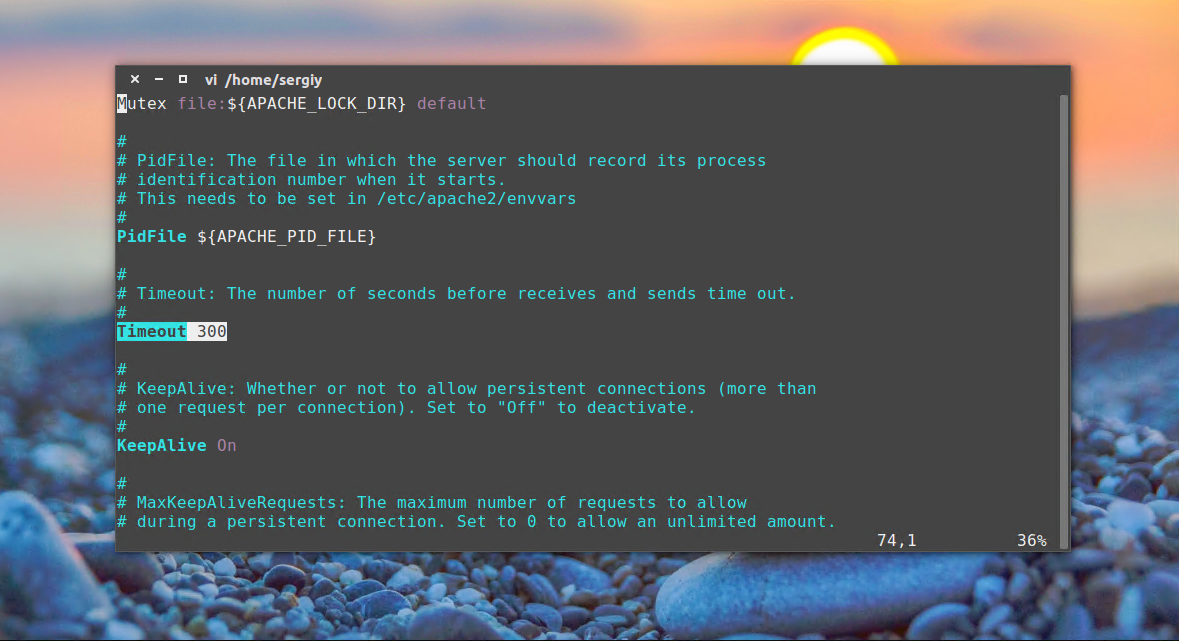
\includegraphics[width=1\textwidth]{imgs/1.4.png}}
    \label{1.4}
\end{figure}
\textbf{Timeout} - указывает как долго сервер будет пытаться продолжить прерванную передачу или прием 
данных. 160 секунд будет вполне достаточно.

\textbf{KeepAlive} On - очень полезный параметр, позволяет передавать\linebreak несколько файлов, за одно 
соединение, например, не только саму html страницу, но и картинки и css файлы.

\textbf{MaxKeepAliveRequests} 100 - максимальное количество запросов за одно соединение, чем больше, тем лучше.

\textbf{KeepAliveTimeout} 5 - таймаут соединения, обычно для загрузки страницы достаточно 5-10 секунд, 
так что больше ставить не нужно, но и рвать соединение раньше чем загрузились все данные тоже не нужно.

\textbf{User, Group} - пользователь и группа, от имени которых будет работать программа.

\textbf{HostnameLookups} - записывать в логи вместо ip адресов доменные имена, лучше отключить, чтобы ускорить работу.

\textbf{LogLevel} - уровень логирования ошибок. По умолчанию используется warn, 
но чтобы логи заполнялись медленнее достаточно включить error

\textbf{Include} - все директивы include отвечают за подключение рассмотренных выше конфигурационных файлов.

\begin{figure}[h]%current location
    \centering
    \scalebox{1}{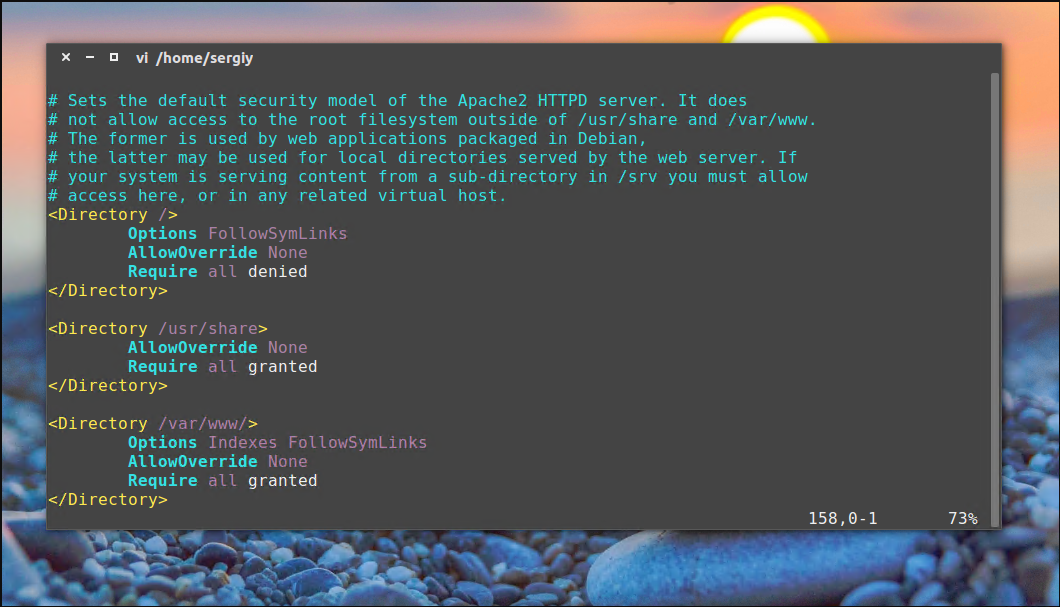
\includegraphics[width=1\textwidth]{imgs/1.5.png}}
    \label{1.5}
\end{figure}

Директивы Directory отвечают за настройку прав доступа к той или иной 
директории в файловой системе. Синтаксис здесь такой:

\begin{lstlisting}
<Directory /адрес/в/файловой/системе/>
Параметр значение
</Directory>
\end{lstlisting}

Здесь доступны такие основные опции:

\textbf{AllowOverride} - указывает нужно ли читать .htaccess файлы из этой директории, это такие 
же файлы настроек и таким же синтаксисом. All - разрешать все, None - не читать эти файлы.

\textbf{DocumentRoot} - устанавливает из какой папки нужно брать документы для отображения пользователю

\textbf{Options} - указывает какие особенности веб-сервера нужно разрешить в этой папке. Например, 
All - разрешить все, FollowSymLinks - переходить по символическим ссылкам, Indexes - отображать 
содержимое каталога если нет файла индекса.

\textbf{Require} - устанавливает, какие пользователи имеют доступ к этому каталогу. Require all 
denied - всем запретить, Require all granted - всем разрешить. можно использовать вместо 
all директиву user или group чтобы явно указать пользователя.

\textbf{Order} - позволяет управлять доступом к директории. Принимает два значения Allow,Deny - 
разрешить для всех, кроме указанных или Deny,Allow - запретить для всех, кроме указанных. 
Теперь мы можем запретить доступ к директории для всех: Deny from all, а затем разрешить 
только для приложения от losst.ru: Allow from losst.ru.

Здесь все эти директивы не используются, поскольку нас устраивают значения по умолчанию, 
но вот в файлах .htaccess они могут быть очень полезны.

У нас остался файл /etc/apache2/ports.conf:
\begin{figure}[h]%current location
    \centering
    \scalebox{1}{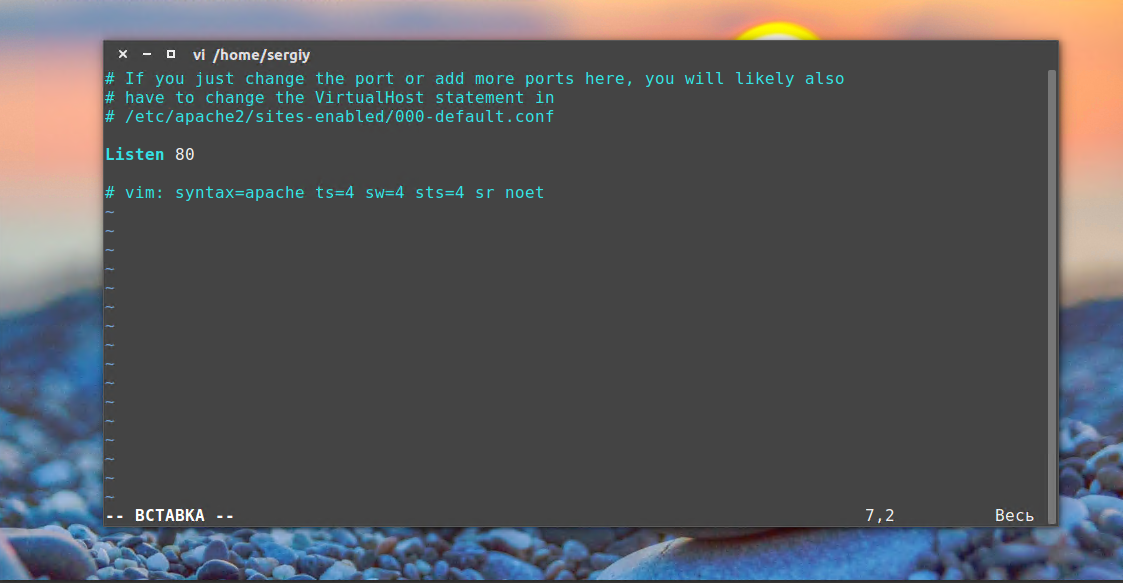
\includegraphics[width=1\textwidth]{imgs/1.6.png}}
    \label{1.6}
\end{figure}
В нем только одна директива, Listen, которая указывает программе на каком порту нужно работать.

Последний файл /etc/apache2/envvars, его вы вряд ли будете использовать, в нем указанны переменные, которые можно использовать в других конфигурационных файлах.
\begin{figure}[h]%current location
    \centering
    \scalebox{1}{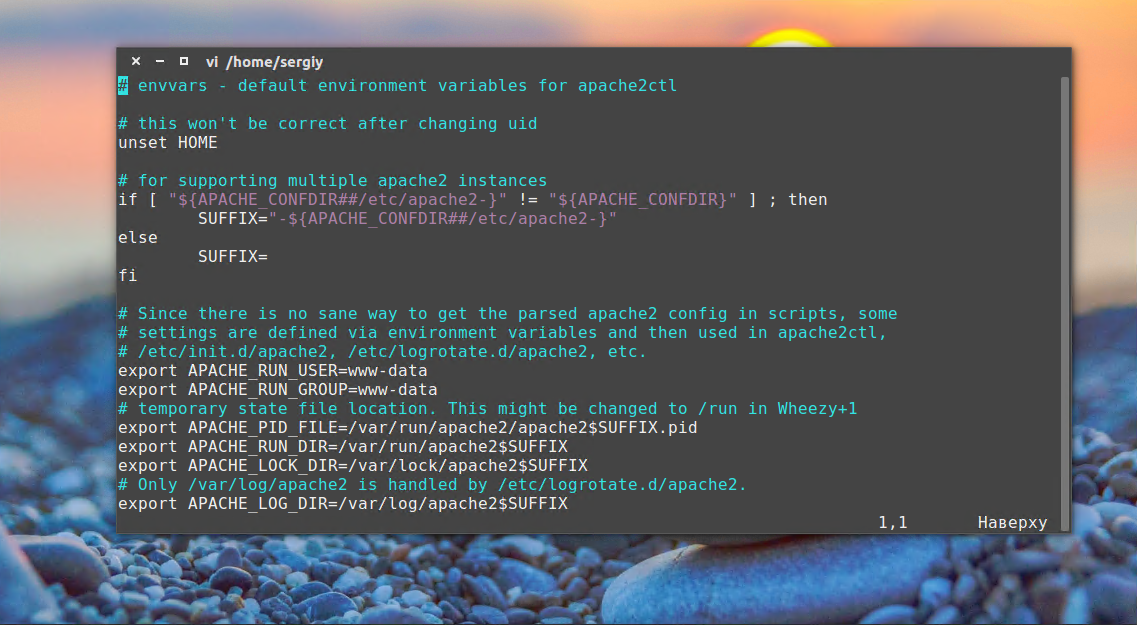
\includegraphics[width=1\textwidth]{imgs/1.7.png}}
    \label{1.7}
\end{figure}


\subsection*{Настройка сервера Apache через htaccess}
\addcontentsline{toc}{subsection}{Настройка сервера Apache через htaccess}
Файлы .htaccess позволяют настраивать веб-сервер на Ubuntu для поведения в определенной директории. 
Все инструкции, указанные в этом файле выполняются как бы они были обвернуты в тег <directory адрес\_папки> 
если бы находились в основном файле.

Важно заметить, что для того, чтобы сервер читал инструкции из .htaccess настройки для 
этой папки в основном файле или файле виртуального хоста не должны содержать \textbf{AllowOverride None}, 
чтобы могли работать все настройки нужно \textbf{AllowOverride All}.

А в остальном, здесь может выполняться любая настройка сервера apache, от включения модулей, 
до обычного изменения доступа к папке. Поскольку все параметры мы уже рассмотрели просто приведем пару примеров:
\begin{lstlisting}
Order Deny,Allow
Deny from all
\end{lstlisting}
Запрещает всем доступ к этой папке, важно применить, для папок с конфигурацией. Чаще всего .htaccess используется для работы с модулем mod\_rewrite, который 
позволяет изменять запросы на лету:
\begin{lstlisting}
RewriteEngine on
RewriteRule ^product/([^/\.]+)/?$ product.php?id=$1 [L]
\end{lstlisting}
Но это очень обширная тема и выходит за рамки этой статьи.


\subsection*{Настройка модулей Apache}
\addcontentsline{toc}{subsection}{Настройка модулей Apache}

Как я уже говорил, Apache - модульная программа, ее функциональность можно расширять с помощью модулей. 
Все доступные модули загрузчики и конфигурационные файлы модулей находятся в папке /etc/apache/mods-available. 
А активированные в /etc/apache/mods-enable.

Но вам необязательно анализировать содержимое этих папок. Настройка Apache 2.4 с помощью добавления 
модулей выполняется с помощью специальных команд. Посмотреть все запущенные модули можно командой:

\begin{lstlisting}
apache2ctl -M
\end{lstlisting}

\begin{figure}[h]%current location
    \centering
    \scalebox{1}{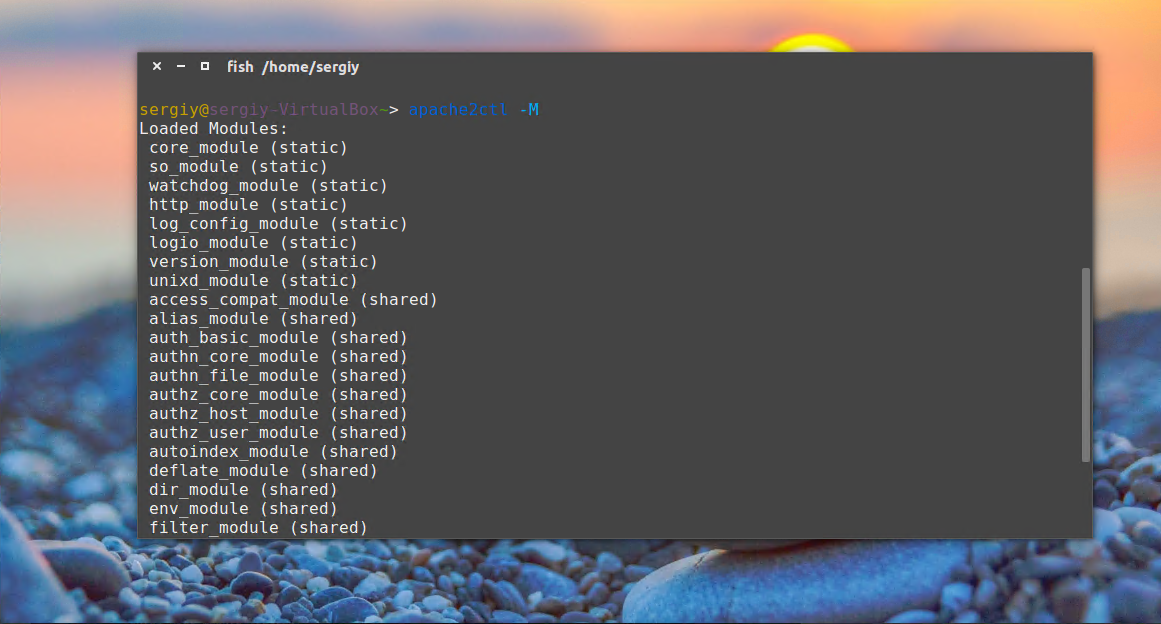
\includegraphics[width=1\textwidth]{imgs/1.8.png}}
    \label{1.8}
\end{figure}

Включить модуль можно командой:
\begin{lstlisting}
sudo a2enmod имя\_модуля
\end{lstlisting}

А отключить:
\begin{lstlisting}
sudo a2dismod имя\_модуля
\end{lstlisting}

После включения или отключения модулей нужно перезагрузить apache:
\begin{lstlisting}
sudo systemctl restart apache2
\end{lstlisting}

Во время выполнения одной из этих команд создается или удаляется символическая ссылка на 
файл модуля с расширением load в директории mods-available. Можете посмотреть содержимое 
этого файла, там только одна строка. Например:
\begin{lstlisting}
vi /etc/apache2/mods-available/deflate.load
\end{lstlisting}
\begin{figure}[H]%current location
    \centering
    \scalebox{1}{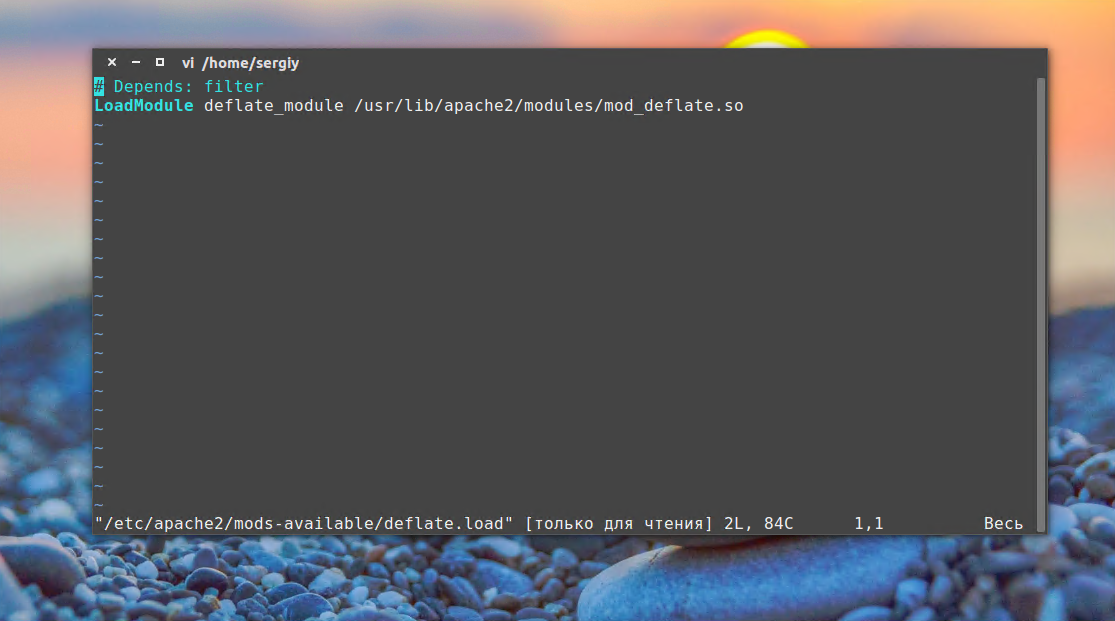
\includegraphics[width=1\textwidth]{imgs/1.9.png}}
    \label{1.9}
\end{figure}
Это к тому, что активировать модуль можно было просто добавив эту строчку в файл apache2.conf.
Но принято делать именно так, чтобы избежать путаницы.

Настройки модулей находятся в той же папке, только в файле с расширением .conf вместо load. 
Например, посмотрим настройки того же модуля для сжатия deflate:
\begin{lstlisting}
vi /etc/apache2/mods-available/deflate.conf
\end{lstlisting}
\begin{figure}[h]%current location
    \centering
    \scalebox{1}{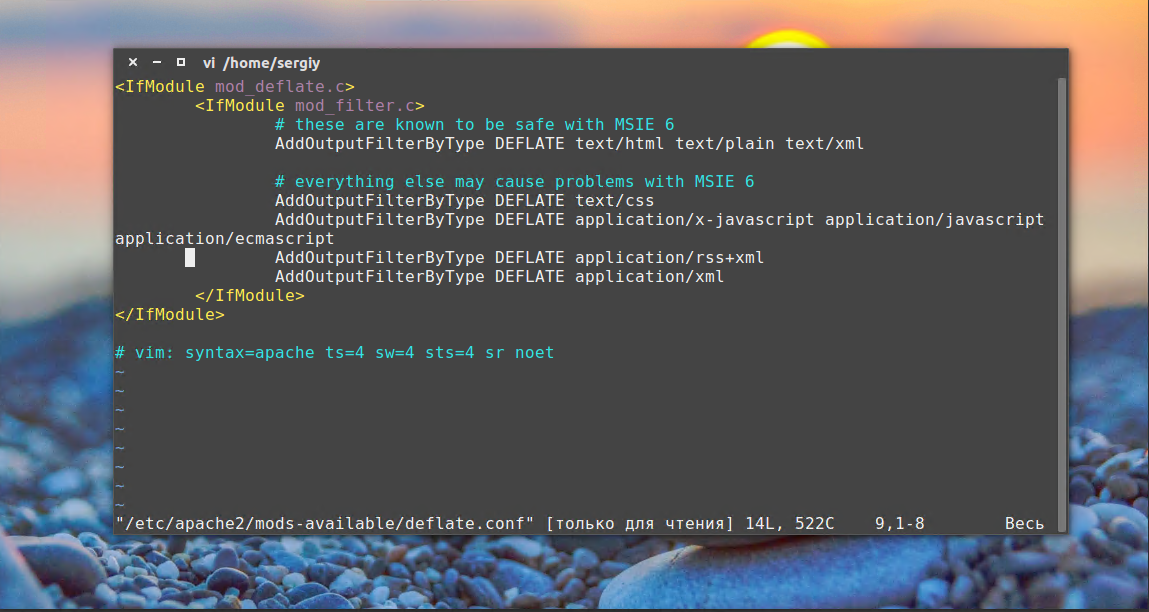
\includegraphics[width=1\textwidth]{imgs/1.10.png}}
    \label{1.10}
\end{figure}
Файлы в папке conf-available, это такие же модули, только они установлены отдельно от apache, это 
может быть конфигурационные файлы для включения модуля php или любого другого языка программирования. 
Здесь работает все точно так же, только команды для включения и отключения этих модулей немного другие:

\begin{lstlisting}
a2enconf имя_модуля
a2disconf имя модуля   
\end{lstlisting}

Как вы убедились, включать модули очень просто. Давайте включим несколько необходимых, 
но не включенных по умолчанию модулей:
\begin{lstlisting}
sudo a2enmod expires
sudo a2enmod headers
sudo a2enmod rewrite
sudo a2enmod ssl
\end{lstlisting}

Модули expires и headers уменьшают нагрузку на сервер. Они возвращают заголовок Not Modified, 
если документ не изменился с последнего запроса. Модуль expiries позволяет устанавливать время, 
на которое браузер должен кэшировать полученный документ. Rewrite позволяет изменять запрашиваемые 
адреса на лету, очень полезно при создании ЧПУ ссылок и т д. А последний для включения поддержки 
шифрования по SSL. Не забудьте перезагрузить apache2 после завершения настроек.


\subsection*{Настройка виртуальных хостов Apache}
\addcontentsline{toc}{subsection}{Настройка виртуальных хостов Apache}
Было бы не совсем удобно, если на одной физической машине можно было размещать только один сайт. 
Apache может поддерживать сотни сайтов на одном компьютере и выдавать для каждого из них правильное 
содержимое. Для этого используются виртуальные хосты. Сервер определяет к какому домену приходит 
запрос и отдает нужное содержимое из папки этого домена.

Настройки хостов Apache расположены в папке \linebreak /etc/apache2/sites-available/. Для создания нового хоста 
достаточно создать файл с любым именем (лучше кончено с именем хоста) и заполнить его нужными данными. 
Обернуть все эти параметры нужно в директиву \textbf{VirtualHost}. Кроме рассмотренных параметров здесь 
будут использоваться такие:

\begin{itemize}
    \item \textbf{ServerName} - основное имя домена
    \item \textbf{ServerAlias} - дополнительное имя, по которому будет доступен сайт
    \item \textbf{ServerAdmin} - электронная почта администратора
    \item \textbf{DocumentRoot} - папка с документами для этого домена\\
\end{itemize}

Например:
\begin{lstlisting}
vi /etc/apache2/sites-available/test.site.conf
\end{lstlisting}

\begin{figure}[h]%current location
    \centering
    \scalebox{1}{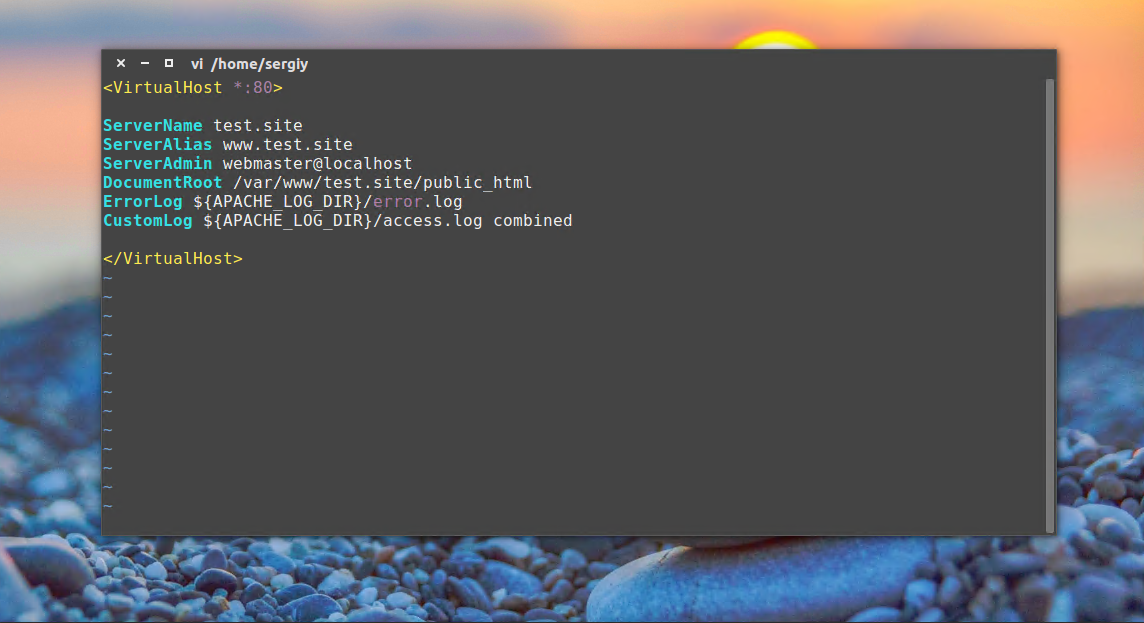
\includegraphics[width=1\textwidth]{imgs/1.11.png}}
    \label{1.11}
\end{figure}

\begin{lstlisting}
<VirtualHost *:80>
ServerName test.site
ServerAlias www.test.site
ServerAdmin webmaster@localhost
DocumentRoot /var/www/test.site/public_html
ErrorLog ${APACHE_LOG_DIR}/error.log
CustomLog ${APACHE_LOG_DIR}/access.log combined
</VirtualHost>
\end{lstlisting}

Виртуальные хосты, как и модули нужно активировать. Для этого есть специальные утилиты. Чтобы активировать наберите:
\begin{lstlisting}
sudo a2ensite test.site
\end{lstlisting}

Здесь test.site - имя файла виртуального хоста. Для отключения тоже есть команда:
\begin{lstlisting}
sudo a2dissite test.site
\end{lstlisting}

Настройка виртуальных хостов Apache завершена и на публичном сервере это все бы уже работало, но 
если вам нужна настройка Apache на домашней машине, то вы ваш новый сайт не откроется в браузере. 
Браузер не знает такого сайта. И откуда ему знать? DNS службы не могут ничего сообщить об этом 
доменном имени. Но в системе Linux мы можем сами указать ip адреса для доменных имен в файле 
/etc/hosts. Поэтому добавляем в конец файла такие строки:
\begin{lstlisting}
vi /etc/hosts
127.0.0.1 test.site
127.0.0.1 www.test.site
\end{lstlisting}

Вот, ну теперь будет работать, открывайте браузер, проверяйте.


\subsubsection*{Шаг 1 — Создание структуры директорий}
\addcontentsline{toc}{subsubsection}{Шаг 1 — Создание структуры директорий}
Прежде всего, нам потребуется создать структуру директорий, где будут храниться данные 
сайтов, которые мы будем выводить посетителям.

Наша корневая директория документов (директория верхнего уровня, где Apache ищет выводимый контент) 
будет задана как отдельные директории в директории /var/www. Здесь мы создадим директории для каждого 
из виртуальных хостов, которые мы планируем создать.

В каждом из этих директорий мы создадим папку public\_html для хранения файлов. 
Это даст нам определенную гибкость в отношении хостинга.

Например, мы будем создавать директории для наших сайтов следующим образом. Если вы используете 
реальные домены или альтернативные значения, замените выделенный текст соответствующим образом.

\begin{lstlisting}
sudo mkdir -p /var/www/example.com/public_html
sudo mkdir -p /var/www/test.com/public_html
\end{lstlisting}

Выделенные красным части представляют доменные имена, которые мы хотим обслуживать через VPS.

\subsubsection*{Шаг 2 — Предоставление разрешений}
\addcontentsline{toc}{subsubsection}{Шаг 2 — Предоставление разрешений}

Теперь у нас имеется структура директорий для наших файлов, но они принадлежат пользователю 
root. Если мы хотим, чтобы обычный пользователь имел возможность изменять файлы в веб-директориях, 
мы можем изменить структуру владения следующим образом:

\begin{lstlisting}
sudo chown -R $USER:$USER /var/www/example.com/public_html
sudo chown -R $USER:$USER /var/www/test.com/public_html
\end{lstlisting}

Переменная \$USER будет принимать значение текущего пользователя в системе при нажатии 
клавиши ENTER. Так наш обычный пользователь теперь является владельцем субдиректорий 
public\_html, где мы будем хранить наш контент.

Также нам необходимо изменять разрешения, чтобы обеспечить доступ для чтения к общей веб-директории 
и всем содержащимся в ней файлам, и папкам, чтобы страницы могли выводиться надлежащим образом:

\begin{lstlisting}
sudo chmod -R 755 /var/www
\end{lstlisting}

Теперь ваш веб-сервер должен иметь необходимые разрешения для вывода контента, а ваш пользователь 
должен иметь права создания контента в соответствующих папках.


\subsubsection*{Шаг 3 — Создание демонстрационных страниц для каждого виртуального хоста}
\addcontentsline{toc}{subsubsection}{Шаг 3 — Создание демонстрационных страниц для каждого виртуального хоста}

Теперь у нас имеется структура директорий. Давайте создадим контент для вывода.

Для демонстрационных целей мы создадим страницу index.html для каждого сайта.

Начнем с example.com. Мы можем открыть файл index.html в текстовом редакторе, в данном случае мы используем nano:

\begin{lstlisting}
nano /var/www/example.com/public_html/index.html
\end{lstlisting}

В этом файле мы создадим документ HTML, указывающий на связанный с ним сайт. Документ 
(/var/www/example.com/public\_html/index.html) будет выглядеть так:

\begin{lstlisting}
<html>
  <head>
    <title>Welcome to Example.com!</title>
  </head>
  <body>
    <h1>Success! The example.com virtual host is working!</h1>
  </body>
</html>
\end{lstlisting}

Сохраните и закройте файл (в nano нажмите CTRL + X, затем Y и ENTER) после завершения редактирования.

Мы можем скопировать этот файл и использовать его в качестве основы для нашего второго сайта:

\begin{lstlisting}
    cp /var/www/example.com/public_html/index.html /var/www/test.com/public_html/index.html
\end{lstlisting}

Затем мы можем открыть файл и изменить соответствующую информацию:

\begin{lstlisting}
nano /var/www/test.com/public_html/index.html
\end{lstlisting}


\begin{lstlisting}
<html>
  <head>
    <title>Welcome to Test.com!</title>
  </head>
  <body> <h1>Success! The test.com virtual host is working!</h1>
  </body>
</html>
\end{lstlisting}

Сохраните и закройте этот файл. Теперь у нас имеются все 
необходимые страницы для тестирования конфигурации виртуальных хостов.


\subsubsection*{Шаг 4 — Создание новых файлов виртуального хоста}
\addcontentsline{toc}{subsubsection}{Шаг 4 — Создание новых файлов виртуального хоста}

Файлы виртуального хоста указывают фактическую конфигурацию виртуальных хостов и задают способ 
ответа веб-сервера Apache на запросы различных доменов.

В Apache имеется файл виртуального хоста по умолчанию с именем 000-default.conf, который мы можем использовать 
в качестве исходной точки. Мы скопируем его для создания файла виртуального хоста для каждого из доменов.

Мы начнем с одного домена, настроим его, скопируем для второго домена и внесем несколько дополнительных 
корректировок. Конфигурация Ubuntu по умолчанию требует, чтобы каждый файл виртуального хоста имел расширение .conf.

Создание первого файла виртуального хоста

Скопируйте файл для первого домена:

\begin{lstlisting}
sudo cp /etc/apache2/sites-available/000-default.conf /etc/apache2/sites-available/example.com.conf
\end{lstlisting}

Откройте новый файл в редакторе с привилегиями root:

\begin{lstlisting}
sudo nano /etc/apache2/sites-available/example.com.conf
\end{lstlisting}

Без комментариев этот файл будет выглядеть примерно так:
\begin{lstlisting}
<VirtualHost *:80>
    ServerAdmin webmaster@localhost
    DocumentRoot /var/www/html
    ErrorLog ${APACHE_LOG_DIR}/error.log
    CustomLog ${APACHE_LOG_DIR}/access.log combined
</VirtualHost>
\end{lstlisting}

В файле мы настроим элементы для нашего первого домена и добавим несколько дополнительных директив. 
Этот раздел виртуального хоста соответствует любым запросам на порт 80, используемый по умолчанию для протокола HTTP.

Вначале нам нужно изменить директиву ServerAdmin на адрес электронной почты, доступный администратору сайта.

\begin{lstlisting}
ServerAdmin admin@example.com
\end{lstlisting}

После этого нам нужно будет добавить две директивы. Директива ServerName задает базовый домен, 
который должен соответствовать этому определению виртуального хоста. Скорее всего, это будет ваш 
домен. Вторая директива под названием ServerAlias определяет дополнительные имена, которые должны 
соответствовать, как если бы они были базовыми. Это полезно для подстановки заданных вами хостов, таких как www:

\begin{lstlisting}
ServerName example.com
ServerAlias www.example.com
\end{lstlisting}

Помимо этого, в нашем файле виртуального хоста нужно изменить только расположение корневой 
директории документов для этого домена. Мы уже создали необходимую нам директорию, так что 
нам нужно изменить директиву DocumentRoot и указать созданную нами директорию:

\begin{lstlisting}
DocumentRoot /var/www/example.com/public_html
\end{lstlisting}

После этого наш файл виртуального хоста \linebreak (/etc/apache2/sites-available/example.com.conf) должен выглядеть следующим образом:

\begin{lstlisting}
<VirtualHost *:80>
ServerAdmin admin@example.com
ServerName example.com
ServerAlias www.example.com
DocumentRoot /var/www/example.com/public_html
ErrorLog ${APACHE_LOG_DIR}/error.log
CustomLog ${APACHE_LOG_DIR}/access.log combined
</VirtualHost>
\end{lstlisting}
Сохраните и закройте файл.

Копирование первого виртуального хоста и настройка для второго домена

Теперь у нас есть первый файл виртуального хоста, и мы можем создать второй файл посредством 
копирования первого и его надлежащей настройки.

Для начала скопируйте файл:
\begin{lstlisting}
sudo cp /etc/apache2/sites-available/example.com.conf /etc/apache2/sites-available/test.com.conf
\end{lstlisting}

Откройте новый файл в редакторе с привилегиями root:
\begin{lstlisting}
sudo nano /etc/apache2/sites-available/test.com.conf 
\end{lstlisting}

Теперь вам нужно изменить все элементы информации, чтобы они ссылались на второй домен. 
После завершения все будет выглядеть следующим образом:

\begin{lstlisting}
<VirtualHost *:80>
ServerAdmin admin@test.com
ServerName test.com
ServerAlias www.test.com
DocumentRoot /var/www/test.com/public_html
ErrorLog ${APACHE_LOG_DIR}/error.log
CustomLog ${APACHE_LOG_DIR}/access.log combined
</VirtualHost>
\end{lstlisting}

Сохраните файл и закройте его после завершения.

\subsubsection*{Шаг 5 — Активация новых файлов виртуального хоста}
\addcontentsline{toc}{subsubsection}{Шаг 5 — Активация новых файлов виртуального хоста}

Мы создали файлы виртуального хоста, и теперь их нужно активировать. В Apache имеются инструменты, 
с помощью которых это можно сделать.

Мы используем инструмент a2ensite для активации каждого из наших сайтов. Дополнительную информацию об 
этом скрипте можно найти в \href{https://manpages.debian.org/jessie/apache2/a2ensite.8.en.html}{документации по a2ensite}.

\begin{lstlisting}
sudo a2ensite example.com.conf
sudo a2ensite test.com.conf
\end{lstlisting}

Отключите сайт по умолчанию, заданный в файле 000-default.conf:

\begin{lstlisting}
sudo a2dissite 000-default.conf
\end{lstlisting}

После завершения нужно перезапустить Apache для вступления изменений в силу и использовать 
команду systemctl status для подтверждения успешного перезапуска.

\begin{lstlisting}
sudo systemctl restart apache2
sudo systemctl status apache2
\end{lstlisting}

Теперь наш сервер должен быть настроен для обслуживания двух сайтов.

\subsubsection*{Шаг 6 — Настройка локального файла hosts (необязательно)}
\addcontentsline{toc}{subsubsection}{Шаг 6 — Настройка локального файла hosts (необязательно)}

Если вы использовали для тестирования этой процедуры фиктивные доменные имена, вы можете проверить 
функциональность этого процесса, временно изменив файл hosts на локальном компьютере.

В результате этого изменения все запросы настроенных доменов будут перехватываться и перенаправляться на сервер 
VPS, как это делала бы система DNS, если бы мы использовали зарегистрированные домены. Это будет работать 
только на локальном компьютере и только для целей тестирования.

Для этих шагов необходимо использовать локальный компьютер, а не сервер VPS. Вам нужно знать 
пароль администратора вашего компьютера или входить в группу администраторов.

Если вы используете компьютер под управлением Mac или Linux, отредактируйте локальный файл с 
привилегиями администратора, введя следующую команду:

\begin{lstlisting}
sudo nano /etc/hosts
\end{lstlisting}

Если вы используете компьютер под управлением Windows, вы \href{https://support.microsoft.com/en-ca/help/923947/you-cannot-modify-the-hosts-file-or-the-lmhosts-file-in-windows-vista}{найдете указания по редактированию файла hosts здесь}.

Вам нужно добавить в файл публичный IP-адрес вашего сервера и доменное имя, которое вы хотите использовать 
для связи с этим сервером.

Для доменов, указанных в настоящем руководстве, замените IP-адрес сервера на your\_server\_IP, и ваш файл 
будет выглядеть примерно так:

\begin{lstlisting}
127.0.0.1   localhost
127.0.1.1   guest-desktop
your_server_IP example.com
your_server_IP test.com
\end{lstlisting}
Сохраните и закройте файл.

При таких настройках все запросы доменов example.com и test.com на нашем компьютере будут 
перенаправляться на наш сервер. Так мы можем протестировать виртуальные хосты, хотя и не 
являемся владельцами этих доменов.

\subsubsection*{Шаг 7 — Тестирование результатов}
\addcontentsline{toc}{subsubsection}{Шаг 7 — Тестирование результатов}

Мы настроили виртуальные хосты и теперь можем протестировать настройки, открыв в браузере настроенные домены:

\begin{lstlisting}
http://example.com
\end{lstlisting}
Вы должны увидеть страницу, выглядящую примерно так:

\begin{figure}[h]%current location
    \centering
    \scalebox{1}{
\includegraphics[width=1\textwidth]{imgs/1.12.png}}
    \label{1.12}
\end{figure}
Также вы можете открыть вторую страницу и увидеть файл, созданный для второго сайта.

\begin{lstlisting}
http://test.com
\end{lstlisting}
\begin{figure}[h]%current location
    \centering
    \scalebox{1}{
\includegraphics[width=1\textwidth]{imgs/1.13.png}}
    \label{1.13}
\end{figure}

Если все эти сайты работают ожидаемым образом, вы успешно настроили \textbf{два} виртуальных хоста на одном сервере

Если вы редактировали файл hosts на своем компьютере, после проверки конфигурации вы можете 
удалить добавленные строки. Так в вашем файле hosts не будет ненужных записей.

Если вам требуется долгосрочный доступ, добавьте доменное имя для каждого необходимого сайта и \href{https://www.digitalocean.com/docs/networking/dns/}{настройте 
его, чтобы оно указывало на ваш сервер}.


\subsubsection*{Заключение}
\addcontentsline{toc}{subsubsection}{Заключение}

Если вы следовали указаниям, теперь у вас должен быть один сервер, обслуживающий два отдельных доменных 
имени. Вы можете добавить дополнительные доменные имена, повторив вышеописанные шаги для создания 
дополнительных виртуальных хостов.

Нет никаких программных ограничений по количеству доменных имен, обслуживаемых Apache, так что вы можете 
создать столько доменных имен, сколько ваш сервер может обслуживать на аппаратном уровне.


\subsection*{\href{https://www.8host.com/blog/keshirovanie-kontenta-pri-pomoshhi-modulej-apache/}{Кэширование котента при помощи модулей Apache}}
\addcontentsline{toc}{subsection}{Кэширование котента при помощи модулей Apache}

\href{https://www.8host.com/blog/keshirovanie-kontenta-pri-pomoshhi-modulej-apache/}
{https://www.8host.com/blog/keshirovanie-kontenta-pri-pomoshhi-modulej-apache/}


\subsection*{Аутентификация и авторизация пользователя}
\addcontentsline{toc}{subsection}{Аутентификация и авторизация пользователя}

\href{https://www.digitalocean.com/community/tutorials/how-to-set-up-password-authentication-with-apache-on-ubuntu-18-04-ru}
{https://www.digitalocean.com/community/tutorials/how-to-set-up-password-authentication-with-apache-on-ubuntu-18-04-ru}




\subsection*{\href{https://www.8host.com/blog/nastrojka-polzovatelskix-stranic-oshibok-apache-v-centos-7/}
{Настройка пользовательских страниц ошибок Apache в CentOS 7}}
\addcontentsline{toc}{subsection}{Настройка пользовательских страниц ошибок Apache в CentOS 7}

При проектировании веб-страниц часто возникает необходимость настроить каждую страницу индивидуально. 
Это касается и страниц ошибок, которые появляются, если запрашиваемый контент по какой-либо причине 
недоступен. В этом руководстве показано, как настроить Apache для отображения пользовательских страниц 
ошибок в системе CentOS 7.

Требования

Для выполнения данного руководства нужна уётная запись пользователя с привилегиями sudo. 
Чтобы настроить такого пользователя, обратитесь к этому руководству. Кроме того, нужно предварительно 
установить Apache; подробные инструкции по установке веб-сервера можно получить здесь.


Создание пользовательской страницы ошибок

Для начала создайте пользовательские страницы ошибок.

\textbf{Примечание}: для тестирования можно использовать следующий код без изменений. Чтобы 
создать свою страницу ошибок, просто замените текст в echo в приведённом ниже коде.

Страницы ошибок будут находиться в каталоге /var/www/html – стандартном каталоге document root 
веб-сервера Apache. Для примера создайте страницу ошибки 404 (по имени custom\_404.html) и общую страницу 
для ошибок 500 (назовите её custom\_50x.html).\newpage

\begin{lstlisting}
echo "<h1 style='color:red'>Error 404: Not found :-(</h1>" | sudo tee /var/www/html/custom_404.html

echo "<p>I have no idea where that file is, sorry.  Are you sure you typed in the correct URL?</p>" | sudo tee -a /var/www/html/custom_404.html

echo "<h1>Oops! Something went wrong...</h1>" | sudo tee /var/www/html/custom_50x.html

echo "<p>We seem to be having some technical difficulties. Hang tight.</p>" | sudo tee -a /var/www/html/custom_50x.html
\end{lstlisting}

Итак, теперь на сервере есть две страницы ошибок.

\subsubsection*{Настройка Apache для отображения пользовательских страниц ошибок}
\addcontentsline{toc}{subsubsection}{Настройка Apache для отображения пользовательских страниц ошибок}

Теперь нужно настроить Apache для поддержки только что созданных страниц в случае возникновения 
соответствующей ошибки. Создайте новый конфигурационный файл в каталоге /etc/httpd/conf.d, который 
хранит настройки для Apache. Назовите файл custom\_errors.conf:

\begin{lstlisting}
sudo nano /etc/httpd/conf.d/custom_errors.conf
\end{lstlisting}
Направьте Apache на соответствующие страницы ошибок.

Для того чтобы связать каждый тип ошибки со специальной страницей ошибок, используйте директиву ErrorDocument. 
В целом, нужно просто указать код состояния HTTP для каждой страницы, и тогда страница появится на экране в 
случае возникновения указанной ошибки.

В данном случае настройки будут выглядеть так:

\begin{lstlisting}
/etc/httpd/conf.d/custom_errors.conf
ErrorDocument 404 /custom_404.html
ErrorDocument 500 /custom_50x.html
ErrorDocument 502 /custom_50x.html
ErrorDocument 503 /custom_50x.html
ErrorDocument 504 /custom_50x.html
\end{lstlisting}

Этих настроек достаточно, чтобы обслуживать пользовательские страницы ошибок.

Однако рекомендуется добавить ещё один блок конфигураций, чтобы клиенты не могли запрашивать 
страницы ошибок напрямую. Это предотвратит путаницу (например, запрошенная напрямую страница ошибки 
будет сообщать пользователю об ошибке, даже если код состояния – 200 (Success)).

Чтобы настроить такое поведение веб-сервера, нужно добавить блок Files для каждой пользовательской 
страницы ошибок. Также нужно проверить, установлена ли переменная окружения REDIRECT\_STATUS; она должна быть 
установлена только если директива ErrorDocument обрабатывает запрос. Если переменная окружения пуста, сервер 
будет обслуживать страницу 404:

\begin{lstlisting}
/etc/httpd/conf.d/custom_errors.conf
ErrorDocument 404 /custom_404.html
ErrorDocument 500 /custom_50x.html
ErrorDocument 502 /custom_50x.html
ErrorDocument 503 /custom_50x.html
ErrorDocument 504 /custom_50x.html
<Files "custom_404.html">
<If "-z %{ENV:REDIRECT_STATUS}">
RedirectMatch 404 ^/custom_404.html$
</If>
</Files>
<Files "custom_50x.html">
<If "-z %{ENV:REDIRECT_STATUS}">
RedirectMatch 404 ^/custom_50x.html$
</If>
</Files>
\end{lstlisting}

Когда страницы ошибок запрашиваются клиентами, возникает ошибка 404, потому что переменная среды не установлена.

\subsubsection*{Тестирование страницы ошибок 500}
\addcontentsline{toc}{subsubsection}{Тестирование страницы ошибок 500}

Проверить работу страницы ошибок 404 очень просто: нужно запросить любой несуществующий контент. 
Чтобы протестировать страниц ошибок 500, нужно создать фиктивный ProxyPass.

Добавьте директиву ProxyPass в конец конфигурационного файла. Отправьте запросы для 
/proxytest на порт 9000 на локальной машине (на этом порте не запущено ни одного сервиса):\pagebreak

\begin{lstlisting}
/etc/httpd/conf.d/custom_errors.conf
ErrorDocument 404 /custom_404.html
ErrorDocument 500 /custom_50x.html
ErrorDocument 502 /custom_50x.html
ErrorDocument 503 /custom_50x.html
ErrorDocument 504 /custom_50x.html
<Files "custom_404.html">
<If "-z %{ENV:REDIRECT_STATUS}">
RedirectMatch 404 ^/custom_404.html$
</If>
</Files>
<Files "custom_50x.html">
<If "-z %{ENV:REDIRECT_STATUS}">
RedirectMatch 404 ^/custom_50x.html$
</If>
</Files>


a2enmod proxy
a2enmod proxy_http
a2enmod proxy_ajp
a2enmod rewrite
a2enmod deflate
a2enmod headers
a2enmod proxy_balancer
a2enmod proxy_connect
a2enmod proxy_html

ProxyPass /proxytest "http://localhost:9000"
\end{lstlisting}

Сохраните и закройте файл.

\subsubsection*{Тестирование страниц ошибок}
\addcontentsline{toc}{subsubsection}{Тестирование страниц ошибок}
Проверьте конфигурационный файл на наличие ошибок:
\begin{lstlisting}
sudo apachectl configtest
\end{lstlisting}

Если команда обнаружила любые ошибки, исправьте их. После этого перезапустите Apache:

\begin{lstlisting}
sudo systemctl restart httpd
\end{lstlisting}

Откройте домен или IP-адрес сервера и запросите несуществующий контент, чтобы проверить работу страницы 404:

\begin{lstlisting}
http://server_domain_or_IP/thiswillerror
\end{lstlisting}

На экране должна появиться страница 404:

\begin{lstlisting}
Error 404: Not found :-(
I have no idea where that file is, sorry.  Are you sure you typed in the correct URL?
\end{lstlisting}

Откройте фиктивный proxypass, чтобы проверить работу страницы 500 (на экране должен появиться код состояния 503 service unavailable):

\begin{lstlisting}
http://server_domain_or_IP/proxytest
\end{lstlisting}

Если всё настроено верно, на экране появится:

\begin{lstlisting}
Oops! Something went wrong...
We seem to be having some technical difficulties. Hang tight.
\end{lstlisting}

После тестирования удалите фиктивную директиву из конфигураций Apache.\newpage


\section*{Заключение}
\addcontentsline{toc}{section}{Заключение}

Итак, теперь на сайте есть уникальные страницы ошибок. Пользовательские страницы ошибок – это отличный способ 
помочь посетителям понять, в чём дело, предоставить им всю необходимую информацию об ошибке и полезные ссылки 
(не забудьте убедиться, что ссылки работают даже в случае возникновения ошибок).

\end{document}